\section*{Part B - Flawed Crypto }

\noindent \begin{center}
\rule[0.5ex]{1\linewidth}{1pt}
\par\end{center}



\noindent \begin{center}
\rule[0.5ex]{1\linewidth}{1pt}
\par\end{center}


\url{https://enterprise.cloudshark.org/blog/packet-capture-of-heartbleed-in-action/}



% the styles for short and long nodes
\tikzset{
short/.style={draw,rectangle,text height=3pt,text depth=13pt,
  text width=7pt,align=center,fill=gray!30},
long/.style={short,text width=1.5cm}
}

% the short nodes \shnode{<label>}{<right of>}{<text>}
\def\shnode#1#2#3{%
  \node[short,right=of #1] (#2) {\rotatebox{270}{#3}}}

% the long nodes \lnode{<label>}{<right of>}
\def\lnode#1#2{%
  \node[long,right=of #1] (#2) {}}

\noindent\begin{tikzpicture}[node distance=-\pgflinewidth]

\node[short,fill=black] (a) {};
\shnode{a}{b}{src};
\shnode{b}{c}{dst};
\shnode{c}{d}{len};
\lnode{d}{e};
\lnode{e}{f};
\node[long,draw=none,fill=none,right=of f,text height=0pt,text depth=0pt,text width=1cm] (g) {$\ldots$};
\node[long,right=of g,label=center:$b$ bits] (h) {};
\lnode{h}{i};
\shnode{i}{j}{len};
\shnode{j}{k}{dst};
\shnode{k}{l}{src};
\node[short,fill=black,right=of l] (m) {};

\node[above right=1cm of a] (ppre) {Packet preamble};
\node[above left=1cm of m] (ppos) {Packet postamble};

\draw[decorate,decoration={brace,raise=2pt}] (b.north west) -- node[above=4pt] {Header} (d.north east);
\draw[decorate,decoration={brace,raise=2pt}] (j.north west) -- node[above=4pt] {Trailer} (l.north east);
\draw[decorate,decoration={brace,raise=2pt}] (h.north west) -- node[above=4pt] {Codeword} (h.north east);
\draw (ppre.west) -- +(-20pt,0pt) -- (a.north);
\draw (ppos.east) -- +(20pt,0pt) -- (m.north);
\draw (a.south east) -- +(0,-1.2cm);
\draw (m.south west) -- +(0,-1.2cm);
\draw[<->] ( $ (a.south east) +(0,-0.6cm) $ ) -- node[fill=white] {$S/B$ Codewords} ( $ (m.south west) +(0,-0.6cm) $ );
\draw[,dotted] (f.north east) -- (h.north west);
\draw[dotted] (f.south east) -- (h.south west);

\end{tikzpicture}



\hskip 5pt
%Here begins the 3d plot
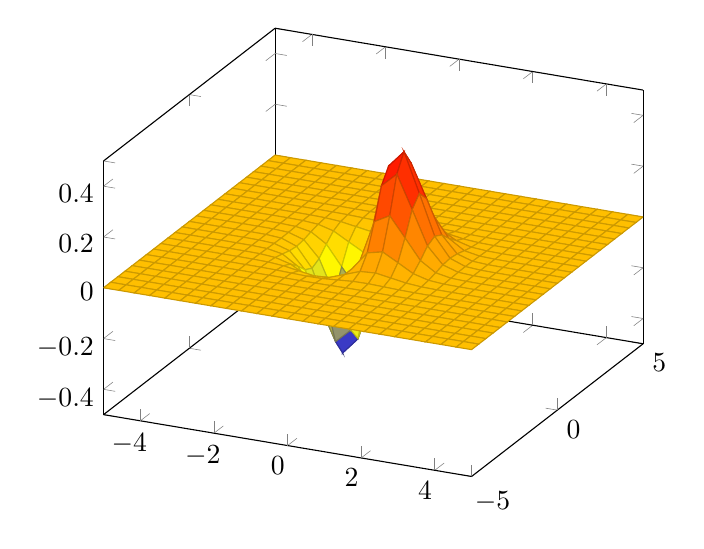
\begin{tikzpicture}
\begin{axis}
\addplot3[
    surf,
]
{exp(-x^2-y^2)*x};
\end{axis}
\end{tikzpicture}